\documentclass[a4paper, 12pt]{article}
\usepackage{vntex}
\usepackage{a4wide,amssymb,epsfig,latexsym,array,hhline,fancyhdr}
\usepackage[normalem]{ulem}
\usepackage[makeroom]{cancel}
\usepackage{amsmath}
\usepackage{longtable}
\usepackage{amsthm}
\usepackage{multicol,longtable,amscd}
\usepackage{diagbox}%Make diagonal lines in tables
\usepackage{booktabs}
\usepackage{alltt}
\usepackage[framemethod=tikz]{mdframed}% For highlighting paragraph backgrounds
\usepackage{caption,subcaption}
\usepackage{lastpage}
\usepackage[lined,boxed,commentsnumbered]{algorithm2e}
\usepackage{enumerate}
\usepackage{color}
\usepackage{xcolor}
\usepackage{graphicx}							% Standard graphics package
\usepackage{array}
\usepackage{tabularx, caption}
\usepackage{multirow}
\usepackage{multicol}
\usepackage{rotating}
\usepackage{graphics}
\usepackage{geometry}
\usepackage{setspace}
\usepackage{epsfig}
\usepackage{tikz}
\usepackage{listings}
\usepackage{float}
\usetikzlibrary{arrows,snakes,backgrounds}
\usepackage{hyperref}
\hypersetup{urlcolor=black,linkcolor=black,citecolor=black,colorlinks=true} 
%\usepackage{pstcol} 								% PSTricks with the standard color package

\newtheorem{theorem}{{\bf Theorem}}
\newtheorem{property}{{\bf Property}}
\newtheorem{proposition}{{\bf Proposition}}
\newtheorem{corollary}[proposition]{{\bf Corollary}}
\newtheorem{lemma}[proposition]{{\bf Lemma}}

\AtBeginDocument{\renewcommand*\contentsname{Mục lục}}
\AtBeginDocument{\renewcommand*\refname{Tài liệu tham khảo}}
\AtBeginDocument{\renewcommand*\listfigurename{Tiêu đề ảnh}}
%\usepackage{fancyhdr}
\setlength{\headheight}{40pt}
\pagestyle{fancy}
\fancyhead{} % clear all header fields
\fancyhead[L]{
 \begin{tabular}{rl}
    \begin{picture}(25,15)(0,0)
    \put(0,-8){
\includegraphics[width=8mm, height=8mm]{hcmut.png}}
   \end{picture}&
	\begin{tabular}{l}
		\textbf{\bf \ttfamily Trường Đại Học Bách Khoa Tp.Hồ Chí Minh}\\
		\textbf{\bf \ttfamily Khoa Khoa Học \& Kỹ Thuật Máy Tính}
	\end{tabular} 	
 \end{tabular}
}
\fancyhead[R]{
	\begin{tabular}{l}
		\tiny \bf \\
		\tiny \bf 
	\end{tabular}  }
\fancyfoot{} % clear all footer fields
\fancyfoot[L]{\scriptsize \ttfamily Báo cáo môn Kiểm tra phần mềm - Học kì 241}
\fancyfoot[R]{\scriptsize \ttfamily Trang {\thepage}/\pageref{LastPage}}
\renewcommand{\headrulewidth}{0.3pt}
\renewcommand{\footrulewidth}{0.3pt}


%%%
\setcounter{secnumdepth}{4}
\setcounter{tocdepth}{3}
\makeatletter
\newcounter {subsubsubsection}[subsubsection]
\renewcommand\thesubsubsubsection{\thesubsubsection .\@alph\c@subsubsubsection}
\newcommand\subsubsubsection{\@startsection{subsubsubsection}{4}{\z@}%
                                     {-3.25ex\@plus -1ex \@minus -.2ex}%
                                     {1.5ex \@plus .2ex}%
                                     {\normalfont\normalsize\bfseries}}
\newcommand*\l@subsubsubsection{\@dottedtocline{3}{10.0em}{4.1em}}
\newcommand*{\subsubsubsectionmark}[1]{}
%\renewcommand{\thesubsubsection}{\alph{subsubsection}}
\everymath{\color{blue}}
\makeatother

\begin{document}

\begin{titlepage}
\begin{center}
VIETNAM NATIONAL UNIVERSITY, HO CHI MINH CITY \\
UNIVERSITY OF TECHNOLOGY \\
FACULTY OF COMPUTER SCIENCE AND ENGINEERING
\end{center}
\vspace{1cm}

\begin{figure}[h!]
\begin{center}

\includegraphics[width=3cm]{hcmut.png}
\end{center}
\end{figure}

\vspace{1cm}


\begin{center}
\begin{tabular}{c}
\multicolumn{1}{l}{\textbf{{\Large KIỂM TRA PHẦN MỀM (CO3015)}}}\\

~~\\
\hline
\\
\\
\textbf{{\Huge BTL 3: AUTOMATION TESTING}}\\
\\

\\
\hline
\end{tabular}
\end{center}

\vspace{3cm}

\begin{table}[h]
\begin{tabular}{rrl}
\hspace{3 cm} & Giảng viên hướng dẫn: & Bùi Hoài Thắng\\

& Sinh viên thực hiện:
& Phạm Đức Hào - 2111128\\
&& Hồ Trọng Nhân - 2111899\\
&& Đậu Đức Quân - 2114531\\
&& Nguyễn Phúc Minh Quân - 2110479\\
&& Trần Mậu Thật - 2112342
\end{tabular}
\end{table}

\begin{center}
{\footnotesize HO CHI MINH CITY, NOVEMBER 2024}
\end{center}
\end{titlepage}


\newpage
\tableofcontents
\newpage

\section{Phân công}
\begin{table}[H]
    \centering
    \begin{longtable}{|p{3cm}|p{3cm}|l|c|}
    \hline 
    Reviewer &
    Validator &
      \multicolumn{1}{c|}{Feature} &Contributon \\ \hline
    Đậu Đức Quân & Trần Mậu Thật & Private file upload \& Private Message& 20\%\\\hline
    Hồ Trọng Nhân & Đậu Đức Quân & Edit Student Name \& Find Course & 20\%\\ \hline
    Nguyễn Phúc Minh Quân & Hồ Trọng Nhân &Create Event \& Change Password&20\%\\ \hline
    Phạm Đức Hào & Nguyễn Phúc Minh Quân & Create Quiz \& Group Message &20\%\\ \hline
    Trần Mậu Thật & Phạm Đức Hào & Post Forum \& Change Score&20\%\\ \hline
    \end{longtable}
    \caption{Bảng phân công công việc}
    \label{tab:my-table}
    \end{table}

\newpage

\section{Giới thiệu}
\subsection{Giới thiệu về công cụ Selenium}

Selenium là một bộ công cụ mã nguồn mở hỗ trợ kiểm thử tự động các ứng dụng web. Ra đời vào năm 2004, Selenium đã trở thành một trong những công cụ phổ biến nhất cho việc kiểm thử giao diện người dùng (UI) nhờ tính linh hoạt, khả năng hỗ trợ đa nền tảng và ngôn ngữ lập trình.

\begin{figure}[H]
    \centering
    
\includegraphics[width=0.5\linewidth]{image/selenium.png}
    \caption{Logo của Selenium}
\end{figure}

Selenium bao gồm nhiều thành phần, nhưng các thành phần chính thường được sử dụng bao gồm:
\begin{itemize}
    \item \textbf{Selenium WebDriver}: Công cụ mạnh mẽ nhất trong bộ Selenium, cho phép thực hiện kiểm thử tự động bằng cách điều khiển trình duyệt một cách trực tiếp.
    \item \textbf{Selenium IDE}: Một tiện ích mở rộng của trình duyệt cho phép ghi lại các kịch bản kiểm thử đơn giản và phát lại chúng.
    \item \textbf{Selenium Grid}: Hỗ trợ chạy kiểm thử song song trên nhiều máy và trình duyệt, tối ưu hóa thời gian kiểm thử.
\end{itemize}

Các tính năng chính của Selenium:
\begin{itemize}
    \item Hỗ trợ đa trình duyệt: Chrome, Firefox, Safari, Edge, v.v.
    \item Tương thích với nhiều ngôn ngữ lập trình: Java, Python, C\#, Ruby, JavaScript.
    \item Được tích hợp tốt với các công cụ kiểm thử và CI/CD như Jenkins, Maven.
\end{itemize}

\subsection{Lý do sử dụng Selenium}

Selenium được lựa chọn làm công cụ kiểm thử tự động trong nhiều dự án vì những lý do sau:
\begin{enumerate}
    \item \textbf{Mã nguồn mở và miễn phí}: Selenium không yêu cầu bất kỳ chi phí bản quyền nào, phù hợp cho cả dự án cá nhân và doanh nghiệp.
    \item \textbf{Hỗ trợ đa nền tảng}: Với Selenium WebDriver, bạn có thể kiểm thử trên nhiều hệ điều hành (Windows, macOS, Linux) và trình duyệt (Chrome, Firefox, Edge, v.v.), đảm bảo tính tương thích của ứng dụng trên các môi trường khác nhau.
    \item \textbf{Khả năng mở rộng cao}: Selenium cung cấp một API mạnh mẽ và linh hoạt, cho phép tích hợp với các framework kiểm thử như TestNG, JUnit (Java), Pytest (Python), hoặc các công cụ như Jenkins, Docker.
    \item \textbf{Hỗ trợ kiểm thử nâng cao}: Selenium không chỉ kiểm thử giao diện mà còn cho phép tương tác với các yếu tố phức tạp trên trang web như các iframe, pop-up, hoặc Ajax.
    \item \textbf{Cộng đồng phát triển lớn}: Với một cộng đồng người dùng rộng lớn, tài liệu phong phú và các diễn đàn hỗ trợ, Selenium giúp người mới dễ dàng học tập và giải quyết các vấn đề phát sinh.
\end{enumerate}

Selenium phù hợp với các dự án yêu cầu kiểm thử tự động ở quy mô lớn, đặc biệt là các ứng dụng web cần đảm bảo hoạt động ổn định trên nhiều môi trường khác nhau.

\subsection{Cấu trúc bài báo cáo}


\section{Description}

\subsection{Create Quiz}
\subsubsection{Level 1}
Ở level 1, mỗi testcase bao gồm các trường:
\begin{itemize}
    \item \textbf{id}: Mã số của testcase.
    \item \textbf{courseName}: Tên khoá học cần tạo bài quiz.
    \item \textbf{quizName}: Tên bài quiz cần tạo.
    \item \textbf{returnButtonText}: Trường text của nút tạo bài quiz.
    \item \textbf{expected}: Phần tử testcase mong đợi sẽ xuất hiện hoặc không xuất hiện.
\end{itemize}

Ví dụ:
\begin{lstlisting}[language=bash, caption={Ví dụ testcase CQ-001-0001 ở level 1}, breaklines=true]
    {
        "id": "CQ-001-0001",
        "courseName": "My first course",
        "quizName": "A",
        "returnButtonText": "Save and return to course",
        "expected": "//div[@data-activityname = 'A']"
    },
\end{lstlisting}
\subsubsection{Level 2}

Ở level 2, mỗi testcase sẽ bao gồm các trường:
\begin{itemize}
    \item \textbf{id}: Mã số của testcase.
    \item \textbf{url}: Đường dẫn đến trang tạo bài quiz.
    \item \textbf{tasks}: Danh sách từng bước cần thực hiện. Mỗi bước bao gồm:
\begin{itemize}
    \item \textbf{action}: Hành động cần thực hiện.
    \item \textbf{element\_type}: Loại định danh (xpath, id, name, link text,...).
    \item \textbf{locator}: Định danh của phần tử cần thao tác.
    \item \textbf{value}: Giá trị cần nhập vào phần tử (nếu có).
\end{itemize}
    \item \textbf{expected}: Kết quả mong đợi. Bao gồm:
\begin{itemize}
    \item \textbf{action}: Hành động cần kiểm tra.
    \item \textbf{element\_type}: Loại định danh (xpath, id, name, link text,...).
    \item \textbf{locator}: Định danh của phần tử cần kiểm tra.
    \item \textbf{value}: Giá trị cần kiểm tra (nếu có).
\end{itemize}
\end{itemize}

Ví dụ:
\begin{lstlisting}[language=bash, caption={Ví dụ testcase CQ-001-0001 ở level 2}, breaklines=true]
{
    "id": "CQ-001-0001",
    "url": "https://sandbox.moodledemo.net/",
    "tasks": [
        {"action": "click", "element_type": "link text", 
            "locator": "Log in", "value": null},
        {"action": "click", "element_type": "id", 
            "locator": "username", "value": null},
        {"action": "send_keys", "element_type": "id", 
            "locator": "username", "value": "teacher"},
        {"action": "click", "element_type": "id", 
            "locator": "password", "value": null},
        {"action": "send_keys", "element_type": "id", 
            "locator": "password", "value": "sandbox24"},
        {"action": "click", "element_type": "id", 
            "locator": "loginbtn", "value": null},
        {"action": "click", "element_type": "link text", 
            "locator": "My courses", "value": null},
        {"action": "click", "element_type": "link text", 
            "locator": "My first course", "value": null, 
            "isOptional": "true"},
        {"action": "toggle", "element_type": "name", 
            "locator": "setmode", "value": "true"}, 
        {"action": "sleep", "element_type": null, 
            "locator": null, "value": 3},  
        
        {"action": "click", "element_type": "xpath", 
            "locator": "//span[contains(.,'Add an activity or resource')]", 
            "value": null},
        {"action": "click", "element_type": "link text", 
            "locator": "Quiz", "value": null},
        {"action": "clear", "element_type": "xpath", 
            "locator": "//*[@id='id_name']", "value": null},
        {"action": "send_keys", "element_type": "xpath", 
            "locator": "//*[@id='id_name']", "value": "A"},

        {"action": "click", "element_type": "xpath", 
            "locator": "//input[@value='Save and return to course']", 
            "value": null},
        {"action": "sleep", "element_type": null, 
            "locator": null, "value": 3}
    ],
    "expected": {
        "action": "is_displayed",
        "element_type": "xpath",
        "locator": "//div[@data-activityname = 'A']",
        "value": "true"
    }
},
\end{lstlisting}
\subsection{Group Message}
\subsubsection{Level 1}
Ở level 1, mỗi testcase bao gồm các trường:
\begin{itemize}
    \item \textbf{id}: Mã số của testcase.
    \item \textbf{groupName}: Tên nhóm cần gửi tin nhắn.
    \item \textbf{messageText}: Nội dung tin nhắn cần gửi.
    \item \textbf{isUserMenu}: Trường xác định xem nút gửi tin nhắn có phải là nút của thanh menu không.
    \item \textbf{expected}: Phần tử testcase mong đợi sẽ không chứa nội dung tin nhắn.
\end{itemize}

Ví dụ:
\begin{lstlisting}[language=bash, caption={Ví dụ testcase GM-001-0001 ở level 1}, breaklines=true]
    {
        "id": "GM-001-0001",
        "groupName": "Team South",
        "messageText": "A",
        "isUserMenu": "true",
        "expected": "//textarea[@aria-label='Write a message...']"
    }
\end{lstlisting}

\subsubsection{Level 2}

Ở level 2, mỗi testcase sẽ bao gồm các trường:
\begin{itemize}
    \item \textbf{id}: Mã số của testcase.
    \item \textbf{url}: Đường dẫn đến trang tạo bài quiz.
    \item \textbf{tasks}: Danh sách từng bước cần thực hiện. Mỗi bước bao gồm:
\begin{itemize}
    \item \textbf{action}: Hành động cần thực hiện.
    \item \textbf{element\_type}: Loại định danh (xpath, id, name, link text,...).
    \item \textbf{locator}: Định danh của phần tử cần thao tác.
    \item \textbf{value}: Giá trị cần nhập vào phần tử (nếu có).
\end{itemize}
    \item \textbf{expected}: Kết quả mong đợi. Bao gồm:
\begin{itemize}
    \item \textbf{action}: Hành động cần kiểm tra.
    \item \textbf{element\_type}: Loại định danh (xpath, id, name, link text,...).
    \item \textbf{locator}: Định danh của phần tử cần kiểm tra.
    \item \textbf{value}: Giá trị cần kiểm tra (nếu có).
\end{itemize}
\end{itemize}

Ví dụ:

\begin{lstlisting}[language=bash, caption={Ví dụ testcase GM-001-0001 ở level 2}, breaklines=true]
    {
    "id": "GM-001-0001",
    "url": "https://school.moodledemo.net/my/courses.php",
    "tasks": [
        {"action": "click", "element_type": "link text", 
            "locator": "Log in", "value": null},
        {"action": "click", "element_type": "id", 
            "locator": "username", "value": null},
        {"action": "send_keys", "element_type": "id", 
            "locator": "username", "value": "student"},
        {"action": "click", "element_type": "id", 
            "locator": "password", "value": null},
        {"action": "send_keys", "element_type": "id", 
            "locator": "password", "value": "moodle2024"},
        {"action": "click", "element_type": "id", 
            "locator": "loginbtn", "value": null},

        {"action": "click", "element_type": "xpath", 
            "locator": "//a[@id='user-menu-toggle']", 
            "value": null},
        {"action": "click", "element_type": "xpath", 
            "locator": "//a[@href='https://school.moodledemo.net/message/index.php']", 
            "value": null},
        {"action": "sleep", "element_type": null, 
            "locator": null, "value": 3},  

        {"action": "click", "element_type": "xpath", 
            "locator": "//span[contains(text(), 'Group')]", 
            "value": null},
        {"action": "click", "element_type": "xpath", 
            "locator": "//strong[contains(text(), 'Team South')]", 
            "value": null},

        {"action": "clear", "element_type": "xpath", 
            "locator": "//textarea[@aria-label='Write a message...']", 
            "value": null},
        {"action": "send_keys", "element_type": "xpath", 
            "locator": "//textarea[@aria-label='Write a message...']", 
            "value": "A"},

        {"action": "click", "element_type": "xpath", 
            "locator": "//i[@class='icon fa-regular fa-paper-plane fa-fw ']", 
            "value": null},
        {"action": "sleep", "element_type": null, 
            "locator": null, "value": 3}
    ],
    "expected": {
        "action": "text",
        "element_type": "xpath",
        "locator": "//textarea[@aria-label='Write a message...']",
        "value": ""
    }
},
\end{lstlisting}


\subsection{Edit Student Name}
\subsubsection{Level 1}
Ở level 1, mỗi testcase bao gồm các trường:
\begin{itemize}
    \item \textbf{last\_name}: Họ mới sẽ được thay đổi
    \item \textbf{first\_name}: .Tên đệm và tên mới sẽ được thay đỏi
    \item \textbf{error\_firstname}: Lỗi đối với ô Tên đệm và tên
    \item \textbf{error\_lastname}: Lỗi đối với ô Họ
\end{itemize}

Ví dụ:
\begin{lstlisting}[language=bash, caption={Ví dụ testcase ESN-001-0002 ở level 1}]
    {
        "last_name": "Smith",
        "first_name": "",
        "error_firstname": "- Xin cho biết tên và tên đệm",
        "error_lastname": ""
    }
\end{lstlisting}
\subsubsection{Level 2}
Ở level 2, mỗi testcase bao gồm các trường:
\begin{itemize}
    \item \textbf{test\_case}: Đánh dấu số thứ tự test case
    \item \textbf{last\_name}: Họ mới sẽ được thay đổi
    \item \textbf{first\_name}: .Tên đệm và tên mới sẽ được thay đỏi
    \item \textbf{error\_firstname}: Lỗi đối với ô Tên đệm và tên
    \item \textbf{error\_lastname}: Lỗi đối với ô Họ
    \item \textbf{step}: Danh sách các bước cần thực hiện. Mỗi bước có thể chứa các trường như sau:
    \begin{itemize}
        \item \textbf{action}: Hành động cần thực hiện
        \item \textbf{url}: Đường dẫn url của trang web
        \item \textbf{width, height}: Kích thước màn hình
        \item \textbf{element\_type}: Loại định danh (xpath, id, name, link text,...)
        \item \textbf{locator}:Định danh của phần tử cần thao tác.
        \item \textbf{value}: Giá trị cần nhập hoặc cần kiểm tra.
    \end{itemize}
\end{itemize}

Ví dụ:
\begin{lstlisting}[language=bash, caption={Ví dụ testcase ESN-001-0001 ở level 2}, breaklines=true]
    {
        "test_case": "Test case 1",
        "last_name": "John",
        "first_name": "Kamala",
        "error_lastname": "",
        "error_firstname": "",
        "steps": [
            {
                "action": "open",
                "url": "https://school.moodledemo.net/?lang=vi"
            },
            {
                "action": "set_window_size",
                "width": 838,
                "height": 816
            },
            {
                "action": "click",
                "elementType": "LINK_TEXT",
                "locator": "Đăng nhập"
            },
            {
                "action": "send_keys",
                "elementType": "ID",
                "locator": "username",
                "value": "student"
            },
            {
                "action": "send_keys",
                "elementType": "ID",
                "locator": "password",
                "value": "moodle2024"
            },
            {
                "action": "click",
                "elementType": "ID",
                "locator": "loginbtn"
            },
            {
                "action": "click",
                "elementType": "ID",
                "locator": "user-menu-toggle"
            },
            {
                "action": "click",
                "elementType": "LINK_TEXT",
                "locator": "Hồ sơ"
            },
            {
                "action": "click",
                "elementType": "LINK_TEXT",
                "locator": "Sửa hồ sơ cá nhân"
            },
            {
                "action": "clear",
                "elementType": "ID",
                "locator": "id_firstname"
            },
            {
                "action": "send_keys",
                "elementType": "ID",
                "locator": "id_firstname",
                "value": "Kamala"
            },
            {
                "action": "clear",
                "elementType": "ID",
                "locator": "id_lastname"
            },
            {
                "action": "send_keys",
                "elementType": "ID",
                "locator": "id_lastname",
                "value": "John"
            },
            {
                "action": "click",
                "elementType": "ID",
                "locator": "id_submitbutton"
            },
            {
                "action": "assert_text",
                "elementType": "CSS_SELECTOR",
                "locator": ".h2",
                "value": "Kamala John"
            }
        ]
    }
\end{lstlisting}
\subsection{Find Course}
\subsubsection{Level 1}
Ở level 1, mỗi testcase bao gồm các trường:
\begin{itemize}
    \item \textbf{str}: Chuỗi được nhập vào ô "Tìm kiếm"
    \item \textbf{list\_course}: Danh sách các khóa học mong đợi sẽ xuất hiện
\end{itemize}

\begin{lstlisting}[language=bash, caption={Ví dụ testcase FC-001-0003 ở level 1}]
    {
        "str": "math",
        "list_course": ["Junior Mathematics"]
    }
\end{lstlisting}
\subsubsection{Level 2}
Ở level 2, mỗi testcase bao gồm các trường:
\begin{itemize}
    \item \textbf{test\_case}: Đánh dấu số thứ tự test case
    \item \textbf{search\_str}: Chuỗi được nhập vào ô "Tìm kiếm"
    \item \textbf{expected\_course}: Danh sách các khóa học mong đợi sẽ xuất hiện
    \item \textbf{step}: Danh sách các bước cần thực hiện. Mỗi bước có thể chứa các trường như sau:
    \begin{itemize}
        \item \textbf{action}: Hành động cần thực hiện
        \item \textbf{url}: Đường dẫn url của trang web
        \item \textbf{width, height}: Kích thước màn hình
        \item \textbf{element\_type}: Loại định danh (xpath, id, name, link text,...)
        \item \textbf{locator}:Định danh của phần tử cần thao tác.
        \item \textbf{value}: Giá trị cần nhập
        \item \textbf{expected}: Gía trị cần kiểm tra
    \end{itemize}
\end{itemize}

\begin{lstlisting}[language=bash, caption={Ví dụ testcase FC-001-0003 ở level 2}, breaklines=true]
    {
        "test_case": "Find Course Test 3",
        "search_str": "math",
        "expected_courses": ["Junior Mathematics"],
        "steps": [
            {
                "action": "open",
                "url": "https://school.moodledemo.net/?lang=vi"
            },
            {
                "action": "set_window_size",
                "width": 838,
                "height": 816
            },
            {
                "action": "click",
                "elementType": "LINK_TEXT",
                "locator": "Đăng nhập"
            },
            {
                "action": "send_keys",
                "elementType": "ID",
                "locator": "username",
                "value": "student"
            },
            {
                "action": "send_keys",
                "elementType": "ID",
                "locator": "password",
                "value": "moodle2024"
            },
            {
                "action": "click",
                "elementType": "ID",
                "locator": "loginbtn"
            },
            {
                "action": "click",
                "elementType": "ID",
                "locator": "groupingdropdown"
            },
            {
                "action": "click",
                "elementType": "CSS_SELECTOR",
                "locator": "a[data-value='all']"
            },
            {
                "action": "click",
                "elementType": "XPATH",
                "locator": "//button[@type='button' and @data-action='limit-toggle']"
            },
            {
                "action": "click",
                "elementType": "LINK_TEXT",
                "locator": "Tất cả"
            },
            {
                "action": "send_keys",
                "elementType": "CSS_SELECTOR",
                "locator": "input[data-region='input'][data-action='search']",
                "value": "math"
            },
            {
                "action": "wait",
                "seconds": 5
            },
            {
                "action": "validate_courses",
                "locator": "//span[contains(@class, 'multiline')]//span[@class='sr-only']",
                "expected": ["Junior Mathematics"]
            }
        ]
    }
\end{lstlisting}

\subsection{Private Message}
\subsubsection{Level 1}
Ở level 1, mỗi testcase bao gồm các trường:
\begin{itemize}
    \item \textbf{id}: Mã số của testcase
    \item \textbf{message}: Nội dung tin nhắn được gửi đi.
    \item \textbf{expected\_text}: Nội dung tin nhắn kết quả để kiếm tra so sánh trùng khớp.
\end{itemize}

\noindent Ví dụ:
\begin{lstlisting}[language=bash, caption={Ví dụ testcase PM-001-0001 ở level 1}, breaklines=true]
    {
      "id": "PM-001-001",
      "message": "ABCDEFMLAKSPQKAMLAMN",
      "expected_text": "ABCDEFMLAKSPQKAMLAMN"
    }
\end{lstlisting}

\subsubsection{Level 2}
Ở level 2, các trường chung bao gồm:

\begin{itemize}
    \item \textbf{url}: Đường dẫn trang web.
    \item \textbf{username}: Tên đăng nhập.
    \item \textbf{password}: Mật khẩu.
\end{itemize}
Tiếp theo là các trường \texttt{selectors} với các giá trị bên trong bao gồm \texttt{type} (ví dụ: ID, XPATH, CSS\_SELECTOR,..) và \texttt{value}. Các \texttt{selectors} ở đây gồm có:
\begin{itemize}
    \item \textbf{login\_link}: Liên kết đăng nhập.
    \item \textbf{username\_input}: Trường nhập tên đăng nhập.
    \item \textbf{password\_input}: Trường nhập mật khẩu.
    \item \textbf{login\_button}: Nút đăng nhập.
    \item \textbf{messaging\_drawer\_toggle}: Nút bật/tắt bảng tin nhắn.
    \item \textbf{messages\_overview\_toggle}: Nút chuyển đổi xem tổng quan tin nhắn.
    \item \textbf{contact\_select}: Lựa chọn liên hệ.
    \item \textbf{message\_input}: Trường nhập tin nhắn.
    \item \textbf{send\_button}: Nút gửi tin nhắn.
    \item \textbf{message\_container}: Vùng chứa tin nhắn.
    \item \textbf{message\_text}: Nội dung tin nhắn.
    \item \textbf{window\_size}: Kích thước cửa sổ.
\end{itemize}

\noindent Tiếp đó là trường \texttt{testcase}, mỗi testcase sẽ có các trường:
\begin{itemize}
    \item \textbf{id}: Mã số của testcase
    \item \textbf{message}: Nội dung tin nhắn được gửi đi.
    \item \textbf{expected\_text}: Nội dung tin nhắn kết quả để kiếm tra so sánh trùng khớp.
\end{itemize}

\noindent Ví dụ:
\begin{lstlisting}[language=bash, breaklines=true]
    "url": "https://school.moodledemo.net/",
    "login_credentials": {
        "username": "amandahamilto205",
        "password": "moodle"
    },
    "selectors": {
        "login_link": {
          "type": "LINK_TEXT",
          "value": "Log in"
        },
        "username_input": {
          "type": "ID",
          "value": "username"
        },
    },
    ...
    "test_cases": [
    {
        "id": "PM-001-001",
        "message": "ABCDEFMLAKSPQKAMLAMN",
        "expected_text": "ABCDEFMLAKSPQKAMLAMN"
    },
\end{lstlisting}

\subsection{Private File Upload}
\subsubsection{Level 1}
Ở level 1, mỗi testcase bao gồm các trường:
\begin{itemize}
    \item \textbf{id}: Mã số của testcase
    \item \textbf{file\_path}: Đường dẫn file từ máy tính. Lấy file từ: \href{https://drive.google.com/drive/folders/1mAcoKv5-AXE3Vms1LvrvOoVR0mKdqAaT?usp=sharing}{Link file test}.
    \item \textbf{expected\_message}: Kết quả thông báo mong đợi sau khi upload file.
\end{itemize}
\noindent Ví dụ:
\begin{lstlisting}[language=bash, breaklines=true]
    {
      "id": "PF-001-002",
      "file_path": "D:\\1byte.txt",
      "expected_message": "Changes saved"
    }
\end{lstlisting}

\subsubsection{Level 2}
Ở level 2, các testcase sẽ có các trường chung như sau:
\begin{itemize}
    \item \textbf{url}: Đường dẫn trang web.
    \item \textbf{window\_size}: Kích thước cửa sổ (bao gồm chiều rộng và chiều cao).
    \item \textbf{credentials}: Thông tin đăng nhập (bao gồm tên người dùng và mật khẩu).
    \item \textbf{selectors}: Các bộ chọn cho các phần tử trên trang web.
    \begin{itemize}
        \item \textbf{login\_link}: Liên kết đăng nhập.
        \item \textbf{username\_field}: Trường nhập tên đăng nhập.
        \item \textbf{password\_field}: Trường nhập mật khẩu.
        \item \textbf{login\_button}: Nút đăng nhập.
        \item \textbf{user\_menu}: Menu người dùng.
        \item \textbf{private\_files}: Tệp riêng tư.
        \item \textbf{add\_file\_button}: Nút thêm tệp.
        \item \textbf{file\_input}: Trường nhập tệp.
        \item \textbf{upload\_button}: Nút tải lên.
        \item \textbf{error\_message}: Thông báo lỗi.
        \item \textbf{submit\_button}: Nút gửi.
        \item \textbf{toast\_message}: Thông báo kiểu toast.
    \end{itemize}
    \item \textbf{timeouts}: Thời gian chờ cho các thao tác.
    \begin{itemize}
        \item \textbf{error\_wait}: Thời gian chờ cho thông báo lỗi.
        \item \textbf{element\_wait}: Thời gian chờ cho phần tử xuất hiện.
        \item \textbf{small\_file\_wait}: Thời gian chờ cho tệp nhỏ.
        \item \textbf{large\_file\_wait}: Thời gian chờ cho tệp lớn.
    \end{itemize}
    \item \textbf{file\_size\_threshold}: Ngưỡng kích thước tệp.
\end{itemize}

\noindent Ví dụ:
\begin{lstlisting}[language=bash, breaklines=true]
      "url": "https://school.moodledemo.net/",
      "window_size": {
        "width": 1296,
        "height": 696
      },
      "credentials": {
        "username": "amandahamilto205",
        "password": "moodle"
      },
      "selectors": {
        "login_link": "Log in",
        "username_field": "username",
        "password_field": "password",
        "login_button": "loginbtn"
        ....
      },
      "timeouts": {
        "error_wait": 3,
        "element_wait": 10,
        "small_file_wait": 15,
        "large_file_wait": 2700
      },
      "file_size_threshold": 90000000,
\end{lstlisting}
\vspace{10pt}
\noindent Tiếp theo đó là tập hợp các testcase như level 1.

\subsection{Create Event}
\subsubsection{Level 1}
Ở level 1, mỗi testcase bao gồm các trường:
\begin{itemize}
    \item \textbf{id}: Mã số của testcase.
    \item \textbf{name}: Tên của sự kiện được tạo ra.
    \item \textbf{startDay}: Ngày bắt đầu của sự kiện.
    \item \textbf{startMonth}: Tháng bắt đầu của sự kiện.
    \item \textbf{startYear}: Năm bắt đầu của sự kiện.
    \item \textbf{startHour}: Giờ bắt đầu của sự kiện.
    \item \textbf{startMinute}: Phút bắt đầu của sự kiện.
    \item \textbf{duration}: Khoảng thời gian sự kiện diễn ra. Khi trường này có giá trị khác null thì các trường kết thúc sự kiện sẽ có giá trị là null và ngược lại.
    \item \textbf{endDay}: Ngày kết thúc của sự kiện.
    \item \textbf{endMonth}: Tháng kết thúc của sự kiện.
    \item \textbf{endYear}: Năm kết thúc của sự kiện.
    \item \textbf{endHour}: Giờ kết thúc của sự kiện.
    \item \textbf{endMinute}: Phút kết thúc của sự kiện.
    \item \textbf{error}: Phần tử testcase mong đợi sẽ xuất hiện khi có lỗi xảy ra.
\end{itemize}

Ví dụ:
\begin{lstlisting}[language=bash, caption={Ví dụ testcase CE-002-004 ở level 1}]
    {
        "id": "CE-002-004",
        "name": "asd",
        "startDay": "20",
        "startMonth": "thang 11",
        "startYear": "2024",
        "startHour": "19",
        "startMinute": "00",
        "duration": null,
        "endDay": "20",
        "endMonth": "thang 11",
        "endYear": "2024",
        "endHour": "18",
        "endMinute": "59",
        "error": "fgroup_id_error_durationgroup"
    }
\end{lstlisting}
\subsubsection{Level 2}
Ở level 2, mỗi testcase bao gồm các trường:
\begin{itemize}
    \item \textbf{id}: Mã số của testcase.
    \item \textbf{url}: Đường dẫn đến trang tạo bài quiz.
    \item \textbf{tasks}: Danh sách từng bước cần thực hiện. Mỗi bước bao gồm:
\begin{itemize}
    \item \textbf{action}: Hành động cần thực hiện.
    \item \textbf{element\_type}: Loại định danh (xpath, id, name, link text,...).
    \item \textbf{locator}: Định danh của phần tử cần thao tác.
    \item \textbf{value}: Giá trị cần nhập vào phần tử (nếu có).
\end{itemize}
    \item \textbf{expected}: Kết quả mong đợi. Bao gồm:
\begin{itemize}
    \item \textbf{action}: Hành động cần kiểm tra.
    \item \textbf{element\_type}: Loại định danh (xpath, id, name, link text, css-selector,...).
    \item \textbf{locator}: Định danh của phần tử cần kiểm tra.
    \item \textbf{value}: Giá trị cần kiểm tra (nếu có).
\end{itemize}
\end{itemize}

Ví dụ:
\begin{lstlisting}[language=bash, caption={Ví dụ testcase CE-002-007 ở level 2}]
    {
        "id": "CE-002-007",
        "url": "https://sandbox.moodledemo.net/",
        "tasks": [
            {"action": "click", "element_type": "id", 
            "locator": "lang-menu-toggle", "value": null},
            {"action": "click", "element_type": "css", 
            "locator": ".dropdown-item:nth-child(103)", "value": null},

            {"action": "click", "element_type": "link text", 
            "locator": "Dang nhap", "value": null},
            {"action": "click", "element_type": "id", 
            "locator": "username", "value": null},
            {"action": "send_keys", "element_type": "id", 
            "locator": "username", "value": "manager"},
            {"action": "click", "element_type": "id", 
            "locator": "password", "value": null},
            {"action": "send_keys", "element_type": "id", 
            "locator": "password", "value": "sandbox24"},
            {"action": "click", "element_type": "id", 
            "locator": "loginbtn", "value": null},

            {"action": "click", "element_type": "link text", 
            "locator": "Bang dieu khien", "value": null},
            {"action": "click", "element_type": "xpath", 
            "locator": "//button[contains(.,'Su kien moi')]", 
            "value": null},

            {"action": "click", "element_type": "id", 
            "locator": "id_name", "value": null},
            {"action": "send_keys", "element_type": "id", 
            "locator": "id_name", "value": "asb"},
            {"action": "send_keys", "element_type": "id", 
            "locator": "id_timestart_day", "value": "20"},
            {"action": "send_keys", "element_type": "id", 
            "locator": "id_timestart_month", "value": "thang 11"},
            {"action": "send_keys", "element_type": "id", 
            "locator": "id_timestart_year", "value": "2024"},
            {"action": "send_keys", "element_type": "id", 
            "locator": "id_timestart_hour", "value": "19"},
            {"action": "send_keys", "element_type": "id", 
            "locator": "id_timestart_minute", "value": "00"},
            
            {"action": "click", "element_type": "xpath", 
            "locator": "//a[contains(.,'Show more...')]", 
            "value": null},

            {"action": "click", "element_type": "css", 
            "locator": ".form-check-inline:nth-child(9)", 
            "value": null},
            {"action": "send_keys", "element_type": "id", 
            "locator": "id_timedurationminutes", "value": "ab"},

            {"action": "click", "element_type": "xpath", 
            "locator": "//button[contains(.,'Luu')]", 
            "value": null}
            
        ],
        "expected": {
            "action" : "is_displayed",
            "element_type": "id",
            "locator": "fgroup_id_error_durationgroup",
            "value": "true"
        }
    }
\end{lstlisting}

\subsection{Change Password}
\subsubsection{Level 1}
Ở level 1, mỗi testcase bao gồm các trường:
\begin{itemize}
    \item \textbf{id}: Mã số của testcase.
    \item \textbf{currentPassword}: Giá trị sẽ nhập vào trường mật khẩu hiện tại.
    \item \textbf{newPassword}: Giá trị sẽ nhập vào trường mật khẩu mới.
    \item \textbf{newPasswordAgain}: Giá trị sẽ nhập vào trường mật khẩu mới (lại).
    \item \textbf{error}: Phần tử testcase mong đợi sẽ xuất hiện khi có lỗi xảy ra.
\end{itemize}

Ví dụ:
\begin{lstlisting}[language=bash, caption={Ví dụ testcase CP-002-001 ở level 1}]
    {
        "id" : "CP-002-001",
        "currentPassword": "sandbox24",
        "newPassword": "a",
        "newPasswordAgain": "a",
        "error" : null
    }
\end{lstlisting}
\subsubsection{Level 2}
Ở level 2, mỗi testcase bao gồm các trường:
\begin{itemize}
    \item \textbf{id}: Mã số của testcase.
    \item \textbf{url}: Đường dẫn đến trang tạo bài quiz.
    \item \textbf{tasks}: Danh sách từng bước cần thực hiện. Mỗi bước bao gồm:
\begin{itemize}
    \item \textbf{action}: Hành động cần thực hiện.
    \item \textbf{element\_type}: Loại định danh (xpath, id, name, link text, css-selector, ...).
    \item \textbf{locator}: Định danh của phần tử cần thao tác.
    \item \textbf{value}: Giá trị cần nhập vào phần tử (nếu có).
\end{itemize}
    \item \textbf{expected}: Kết quả mong đợi. Bao gồm:
\begin{itemize}
    \item \textbf{action}: Hành động cần kiểm tra.
    \item \textbf{element\_type}: Loại định danh (xpath, id, name, link text,...).
    \item \textbf{locator}: Định danh của phần tử cần kiểm tra.
    \item \textbf{value}: Giá trị cần kiểm tra (nếu có).
\end{itemize}
\end{itemize}

Ví dụ:
\begin{lstlisting}[language=bash, caption={Ví dụ testcase CP-002-004 ở level 2}]
    {
        "id": "CP-002-004",
        "url": "https://sandbox.moodledemo.net/",
        "tasks": [
            {"action": "click", "element_type": "id", 
            "locator": "lang-menu-toggle", "value": null},
            {"action": "click", "element_type": "css", 
            "locator": ".dropdown-item:nth-child(103)", 
            "value": null},

            {"action": "click", "element_type": "link text", 
            "locator": "Dang nhap", "value": null},
            {"action": "click", "element_type": "id", 
            "locator": "username", "value": null},
            {"action": "send_keys", "element_type": "id", 
            "locator": "username", "value": "student"},
            {"action": "click", "element_type": "id", 
            "locator": "password", "value": null},
            {"action": "send_keys", "element_type": "id", 
            "locator": "password", "value": "a"},
            {"action": "click", "element_type": "id", 
            "locator": "loginbtn", "value": null},

            {"action": "click", "element_type": "id", 
            "locator": "user-menu-toggle", "value": null},
            {"action": "click", "element_type": "link text", 
            "locator": "Tuy chon", "value": null},
            {"action": "click", "element_type": "link text", 
            "locator": "Doi mat khau", "value": null},

            {"action": "send_keys", "element_type": "id", 
            "locator": "id_password", "value": "a"},
            {"action": "send_keys", "element_type": "id", 
            "locator": "id_newpassword1", "value": "a"},
            {"action": "send_keys", "element_type": "id", 
            "locator": "id_newpassword2", "value": "b"},

            {"action": "click", "element_type": "id", 
            "locator": "id_submitbutton", "value": null}
            
        ],
        "expected": {
            "action" : "is_displayed",
            "element_type": "id",
            "locator": "id_error_newpassword1",
            "value": "true"
        }
    }
\end{lstlisting}


\subsection{Message Forum}
\subsubsection{Level 1}
Ở level 1, mỗi testcase bao gồm các trường:
\begin{itemize}
    \item \textbf{id}: Mã số của testcase.
    \item \textbf{subject}: Chủ đề của thông báo cần gửi vào forum, tiêu đề
    \item \textbf{message}: Nội dung của thông báo cần gửi vào forum
    \item \textbf{error}: Trả về mã lỗi không mong đợi, hoặc kết quả nếu thành công
\end{itemize}

Ví dụ:
\begin{lstlisting}[language=bash, caption={Ví dụ testcase MF-1-001 ở level 1}]
    {
    "id": "MF-1-001",
    "subject" : "Assignment Submit Date",
    "message" : "Before 24/11/2024",
    "error": "user-notifications"  
  }
\end{lstlisting}
\subsubsection{Level 2}

Ở level 2, mỗi testcase sẽ bao gồm các trường:
\begin{itemize}
    \item \textbf{id}: Mã số của testcase.
    \item \textbf{url}: Đường dẫn đến trang chủ của khoá học.
    \item \textbf{tasks}: Danh sách từng bước cần thực hiện. Mỗi bước bao gồm:
\begin{itemize}
    \item \textbf{action}: Hành động cần thực hiện.
    \item \textbf{element\_type}: Loại định danh (xpath, id, name, link text,...).
    \item \textbf{locator}: Định danh của phần tử cần thao tác.
    \item \textbf{value}: Giá trị cần nhập vào phần tử (nếu có).
\end{itemize}
    \item \textbf{expected}: Kết quả mong đợi. Bao gồm:
\begin{itemize}
    \item \textbf{action}: Hành động cần kiểm tra.
    \item \textbf{element\_type}: Loại định danh (xpath, id, name, link text,...).
    \item \textbf{locator}: Định danh của phần tử cần kiểm tra.
    \item \textbf{value}: Giá trị cần kiểm tra (nếu có).
\end{itemize}
\end{itemize}

Ví dụ:
\begin{lstlisting}[language=bash, caption={Ví dụ testcase MF-1-001 ở level 2}, breaklines=true]
    {
        "id": "MF-1-001",
        "url": "https://school.moodledemo.net/",
        "tasks": [
            {"action": "click", "element_type": "id", "locator": "lang-menu-toggle", "value": null},
            {"action": "scroll", "element_type": "xpath", "locator": "//*[@id='lang-action-menu']/a[101]", "value": null},
            {"action": "click", "element_type": "xpath", "locator": "//*[@id='lang-action-menu']/a[101]", "value": null},
            {"action": "click", "element_type": "link text", "locator": "Đăng nhập", "value": null},
            {"action": "send_keys", "element_type": "id", "locator": "username", "value": "teacher"},
            {"action": "click", "element_type": "id", "locator": "password", "value": null},
            {"action": "send_keys", "element_type": "id", "locator": "password", "value": "moodle2024"},
            {"action": "click", "element_type": "id", "locator": "loginbtn", "value": null},

            {"action": "click", "element_type": "link text", "locator": "Mindful course creation", "value": null},
            {"action": "scroll", "element_type": "xpath", "locator": "//*[@id='module-967']/div/div[2]/div[2]/div/div/a", "value": null},
            {"action": "click", "element_type": "xpath", "locator": "//*[@id='module-967']/div/div[2]/div[2]/div/div/a", "value": null},

            {"action": "refresh", "element_type": "", "locator": "", "value": null},
            

            {"action": "scroll", "element_type": "xpath", "locator": "//*[@id='region-main']/div[2]/div[1]/div/div[2]/a", "value": null},
            {"action": "click", "element_type": "xpath", "locator": "//*[@id='region-main']/div[2]/div[1]/div/div[2]/a", "value": null},

            {"action": "scroll", "element_type": "id", "locator": "id_subject", "value": null},
            {"action": "send_keys", "element_type": "id", "locator": "id_subject", "value": "Assignment Submit Date"},
            
            

            {"action": "switch", "element_type": "xpath", "locator": "//*[@id='id_message_ifr']", "value": null},

            {"action": "send_keys", "element_type": "id", "locator": "tinymce", "value": "Before 24/11/2024"},
            {"action": "switch_default", "element_type": "", "locator": null, "value": null},

            {"action": "scroll", "element_type": "id", "locator": "id_submitbutton", "value": null},
            {"action": "click", "element_type": "id", "locator": "id_submitbutton", "value": null}
            
        ],
        "expected": {
            "action" : "is_displayed",
            "element_type": "id",
            "locator": "user-notifications",
            "value": "true"
        }
    }
\end{lstlisting}
\subsection{Edit Score}
\subsubsection{Level 1}
Ở level 1, mỗi testcase bao gồm các trường:
\begin{itemize}
    \item \textbf{id}: Mã số của testcase.
    \item \textbf{score}: Điểm dùng để chỉnh sửa cho sinh viên
    \item \textbf{error}: Mã lỗi thông báo lỗi, hoặc là null nếu thành công.
\end{itemize}

Ví dụ:
\begin{lstlisting}[language=bash, caption={Ví dụ testcase ES-1-001 ở level 1}]
    {
        "id": "ES-1-001",
        "score" : "",
        "error": null  
    },
\end{lstlisting}

\subsubsection{Level 2}

Ở level 2, mỗi testcase sẽ bao gồm các trường:
\begin{itemize}
    \item \textbf{id}: Mã số của testcase.
    \item \textbf{url}: Đường dẫn đến trang chủ các khoá học.
    \item \textbf{tasks}: Danh sách từng bước cần thực hiện. Mỗi bước bao gồm:
\begin{itemize}
    \item \textbf{action}: Hành động cần thực hiện.
    \item \textbf{element\_type}: Loại định danh (xpath, id, name, link text,...).
    \item \textbf{locator}: Định danh của phần tử cần thao tác.
    \item \textbf{value}: Giá trị cần nhập vào phần tử (nếu có).
\end{itemize}
    \item \textbf{expected}: Kết quả mong đợi. Bao gồm:
\begin{itemize}
    \item \textbf{action}: Hành động cần kiểm tra.
    \item \textbf{element\_type}: Loại định danh (xpath, id, name, link text,...).
    \item \textbf{locator}: Định danh của phần tử cần kiểm tra.
    \item \textbf{value}: Giá trị cần kiểm tra (nếu có).
\end{itemize}
\end{itemize}

Ví dụ:

\begin{lstlisting}[language=bash, caption={Ví dụ testcase  ES-1-001 ở level 2}, breaklines=true]
    {
        "id": "ES-1-001",
        "url": "https://school.moodledemo.net/",
        "tasks": [
            {"action": "click", "element_type": "id", "locator": "lang-menu-toggle", "value": null},
            {"action": "scroll", "element_type": "xpath", "locator": "//*[@id='lang-action-menu']/a[101]", "value": null},
            {"action": "click", "element_type": "xpath", "locator": "//*[@id='lang-action-menu']/a[101]", "value": null},
            {"action": "click", "element_type": "link text", "locator": "Đăng nhập", "value": null},
            {"action": "send_keys", "element_type": "id", "locator": "username", "value": "teacher"},
            {"action": "click", "element_type": "id", "locator": "password", "value": null},
            {"action": "send_keys", "element_type": "id", "locator": "password", "value": "moodle2024"},
            {"action": "click", "element_type": "id", "locator": "loginbtn", "value": null},

            {"action": "click", "element_type": "link text", "locator": "Mindful course creation", "value": null},
            {"action": "click", "element_type": "link text", "locator": "Điểm số", "value": null},
            {"action": "close_modal", "element_type": "", "locator": "", "value": null},

            {"action": "click", "element_type": "xpath", "locator": "//*[@id='usernavigation']/form", "value": null},

            {"action": "scroll", "element_type": "id", "locator": "grade_14_490", "value": null},
            {"action": "send_keys", "element_type": "id", "locator": "grade_14_490", "value": ""},

            {"action": "click", "element_type": "id", "locator": "gradersubmit", "value": null},

            {"action": "sleep", "element_type": "", "locator": "", "value": 3}
                       
        ],
        "expected": {
            "action" : "text",
            "element_type": "id",
            "locator": "grade_14_490",
            "value": ""
        }
    }
\end{lstlisting}

\section{Results}

\subsection{Create Quiz}

\begin{figure}[H]
\centering
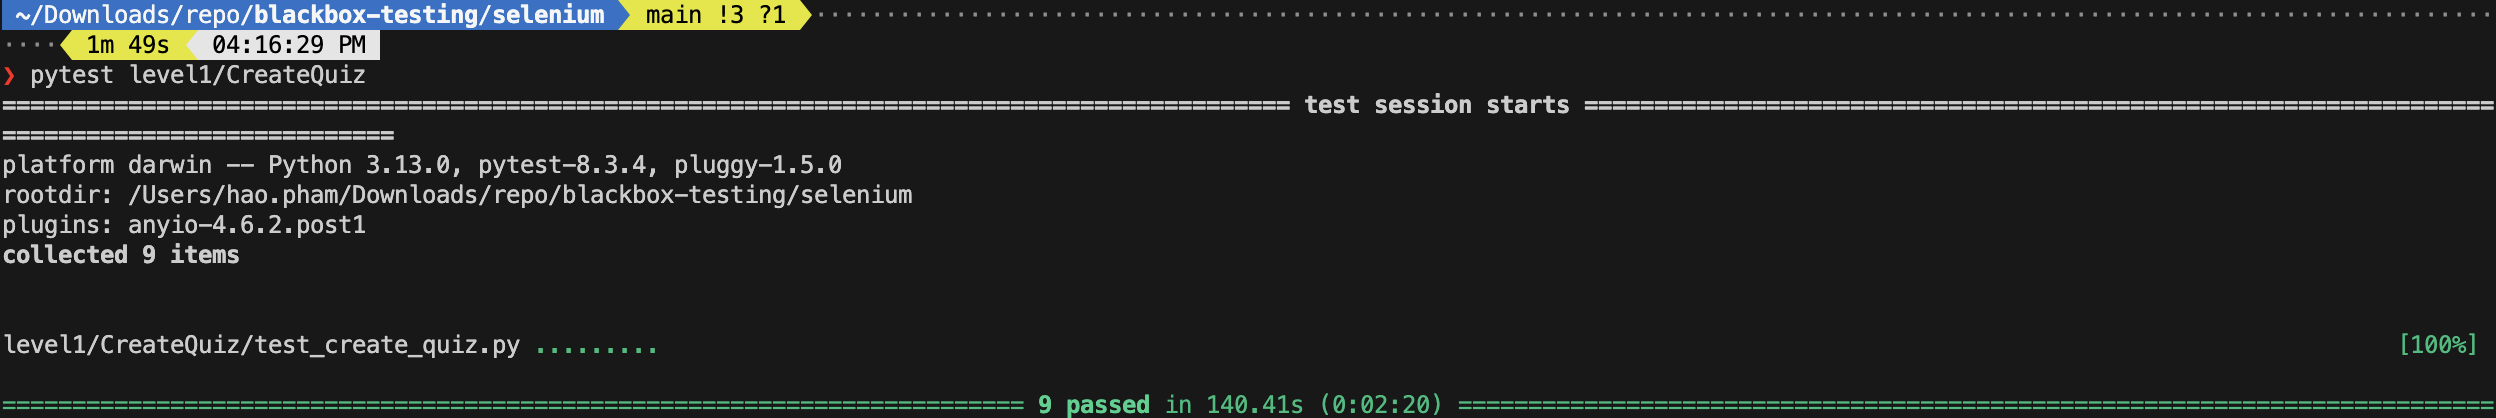
\includegraphics[width=\linewidth]{image/results-create-quiz.png}
\caption{Kết quả kiểm thử chức năng Create Quiz}
\end{figure}

\subsection{Group Message}

\begin{figure}[H]
    \centering
    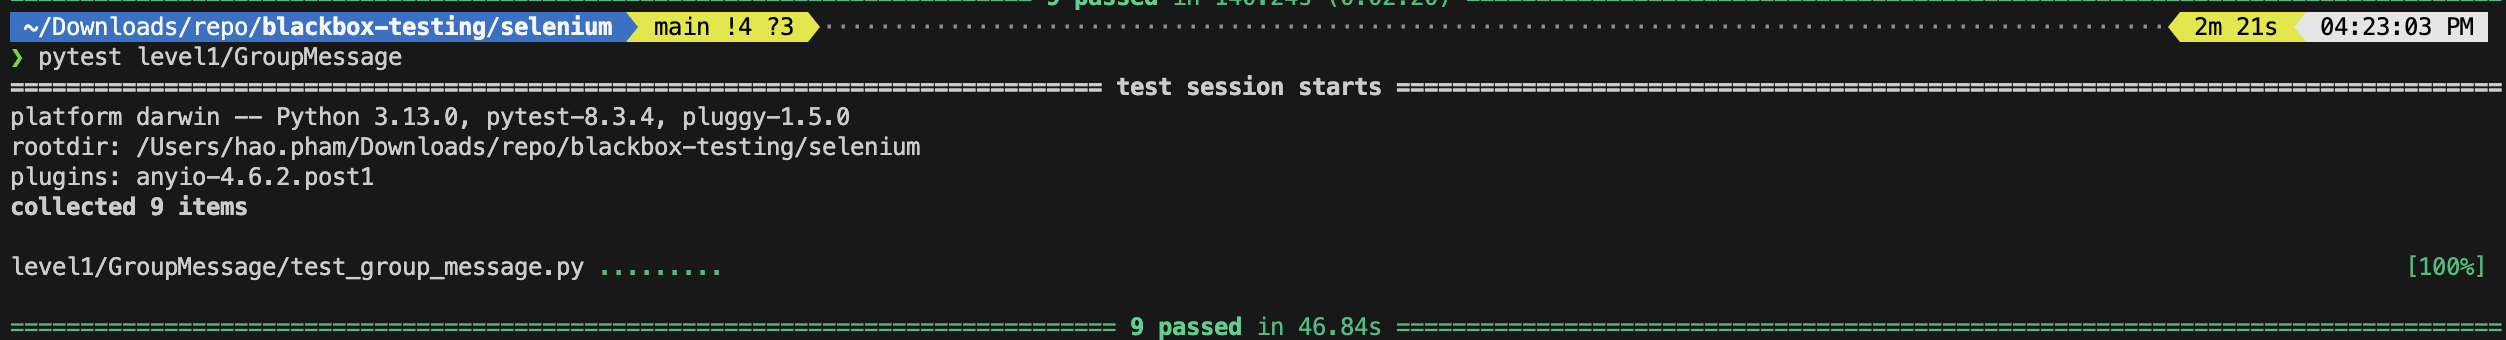
\includegraphics[width=\linewidth]{image/results-group-message.png}
    \caption{Kết quả kiểm thử chức năng Group Message}
\end{figure}

\subsection{Edit Student Name}
\begin{figure}[H]
\centering
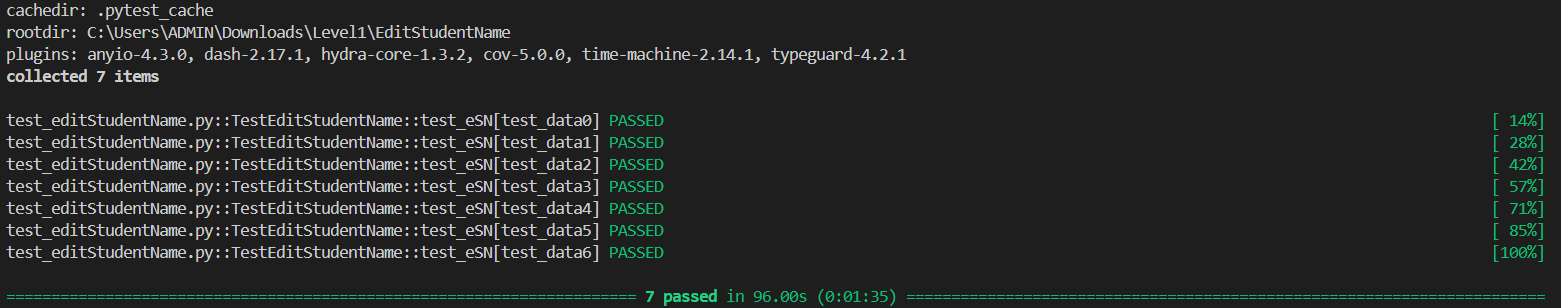
\includegraphics[width=\linewidth]{image/edit-student-name.png}
\caption{Kết quả kiểm thử chức năng Edit Student Name}
\end{figure}
\subsection{Find Course}
\begin{figure}[H]
\centering
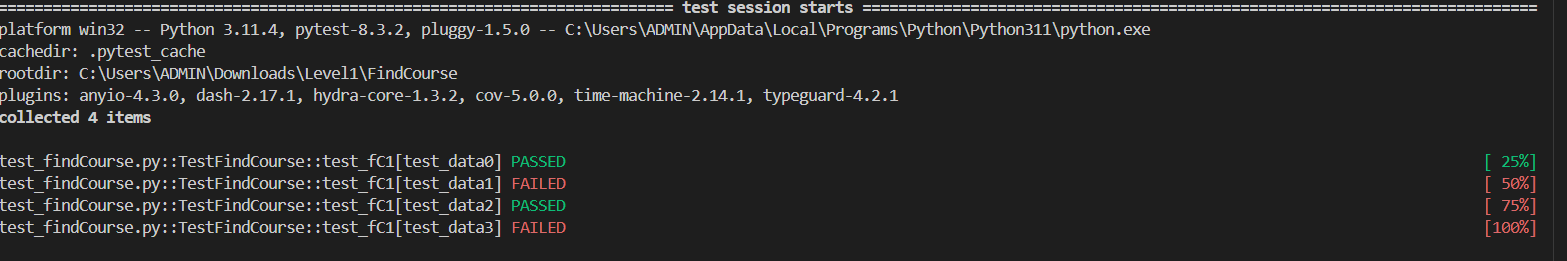
\includegraphics[width=\linewidth]{image/result_find_course.png}
\caption{Kết quả kiểm thử chức năng Find Course}
\end{figure}

Hai test case Failed bao gồm test case với chuỗi tìm kiếm không có khóa học phù hợp và chuỗi tìm kiếm chỉ gồm một kí tự

\subsection{Private message}
\subsubsection{Level 1}
\begin{figure}[H]
    \centering
    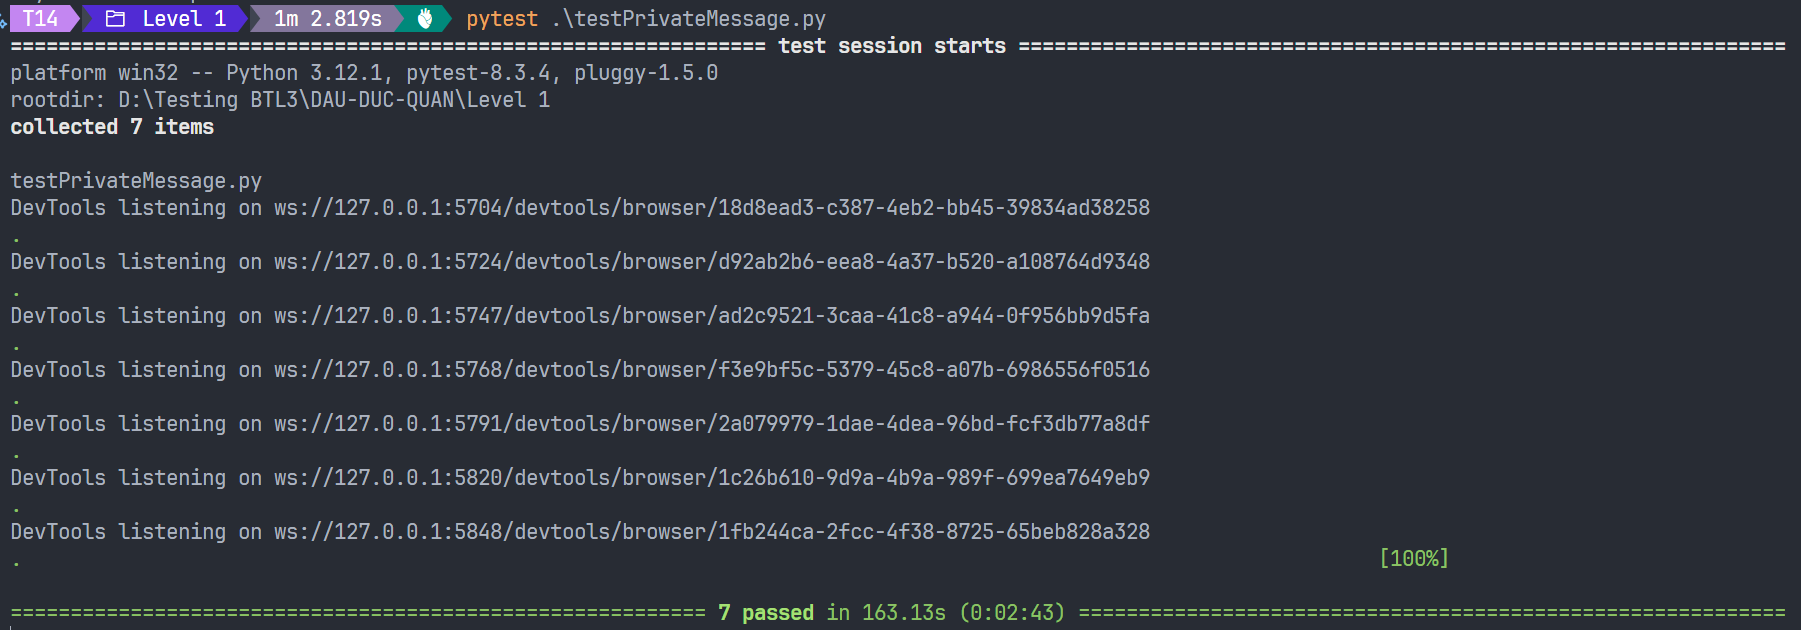
\includegraphics[width=0.8\linewidth]{image/pm_lv1.png}
    \caption{Kết quả kiểm thử chức năng Private message ở Level 1}
\end{figure}

\subsubsection{Level 2}
\begin{figure}[H]
    \centering
    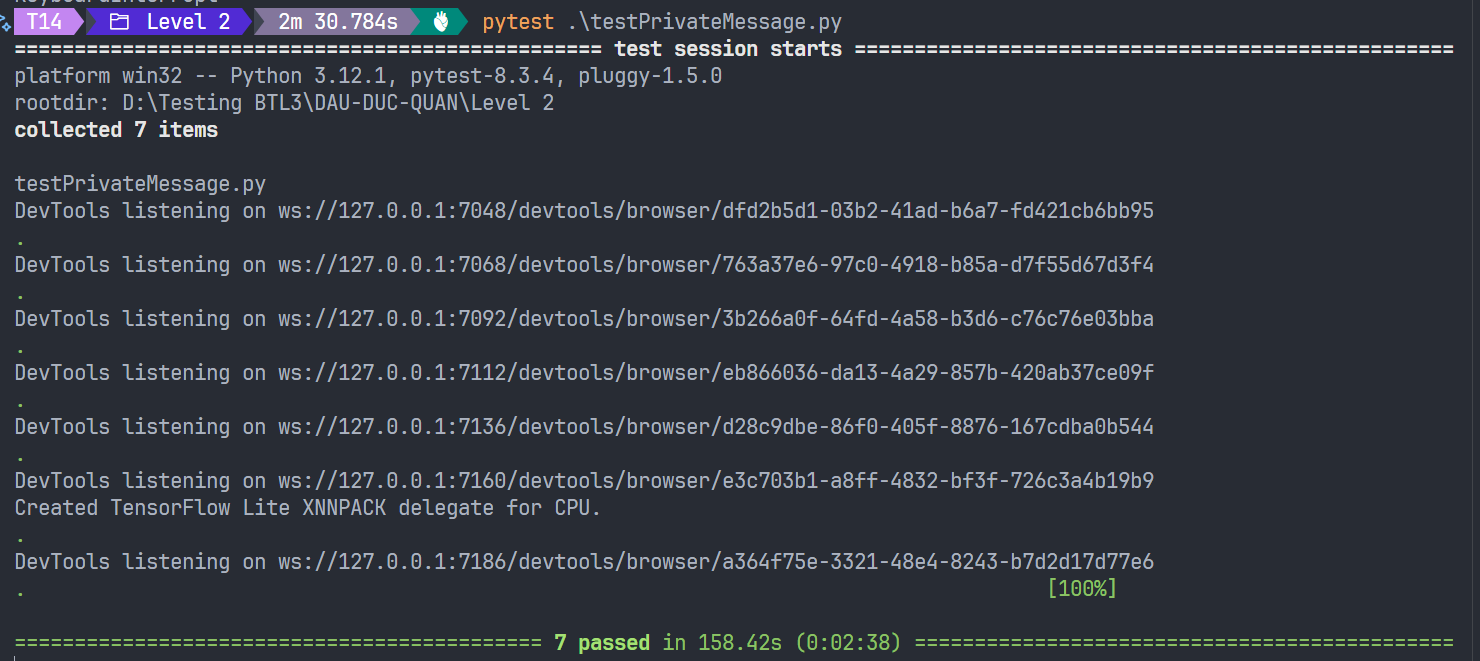
\includegraphics[width=0.8\linewidth]{image/pm_lv2.png}
    \caption{Kết quả kiểm thử chức năng Private message ở Level 2}
\end{figure}

\subsection{Private file upload}
\subsubsection{Level 1}
\begin{figure}[H]
    \centering
    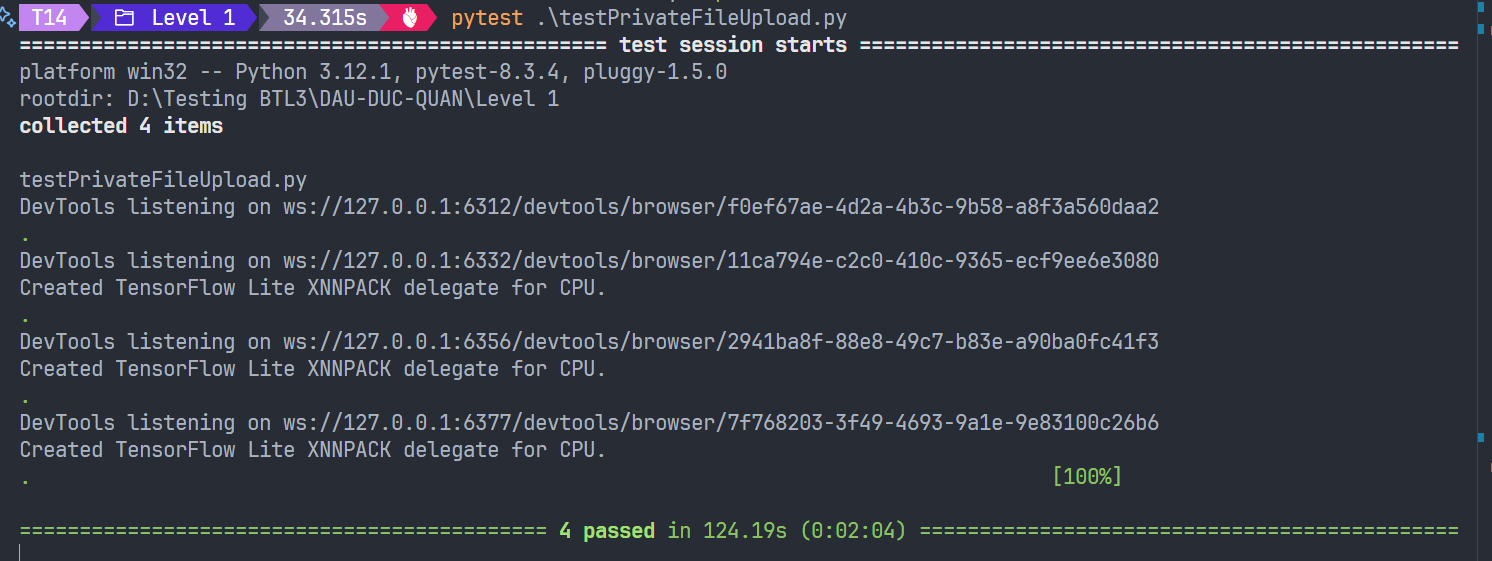
\includegraphics[width=0.8\linewidth]{image/pf_lv1.png}
    \caption{Kết quả kiểm thử chức năng Private file upload ở Level 1}
\end{figure}

\subsubsection{Level 2}
\begin{figure}[H]
    \centering
    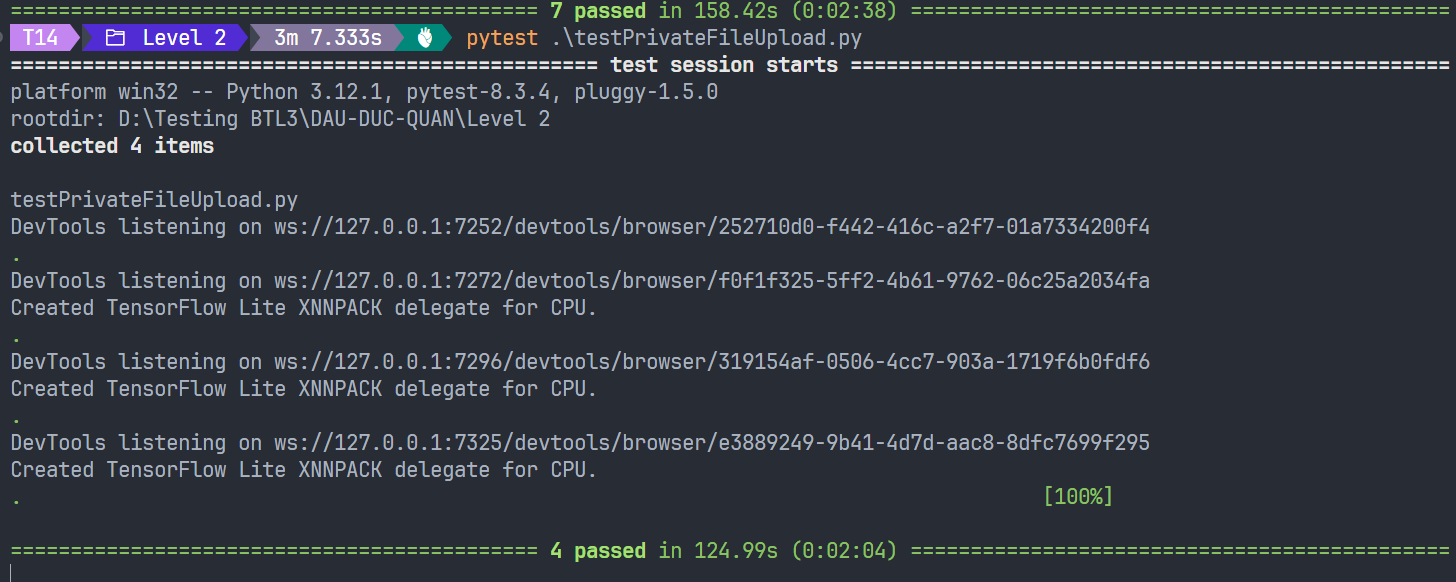
\includegraphics[width=0.8\linewidth]{image/pf_lv2.png}
    \caption{Kết quả kiểm thử chức năng Private file upload ở Level 2}
\end{figure}


\subsection{Create Event}
\subsubsection{Level 1}
\begin{figure}[H]
    \centering
    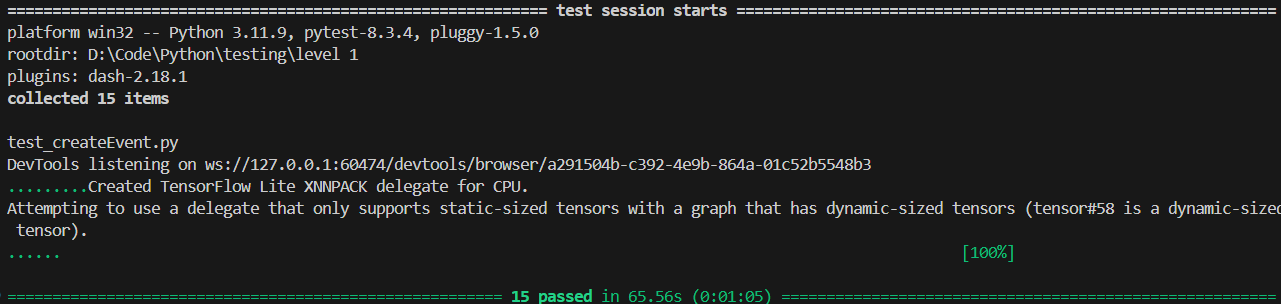
\includegraphics[width=0.8\linewidth]{image/results-create-event-lv1.png}
    \caption{Kết quả kiểm thử chức năng Create Event ở Level 1}
    \label{fig:enter-label}
\end{figure}
\subsubsection{Level 2}
\begin{figure}[H]
    \centering
    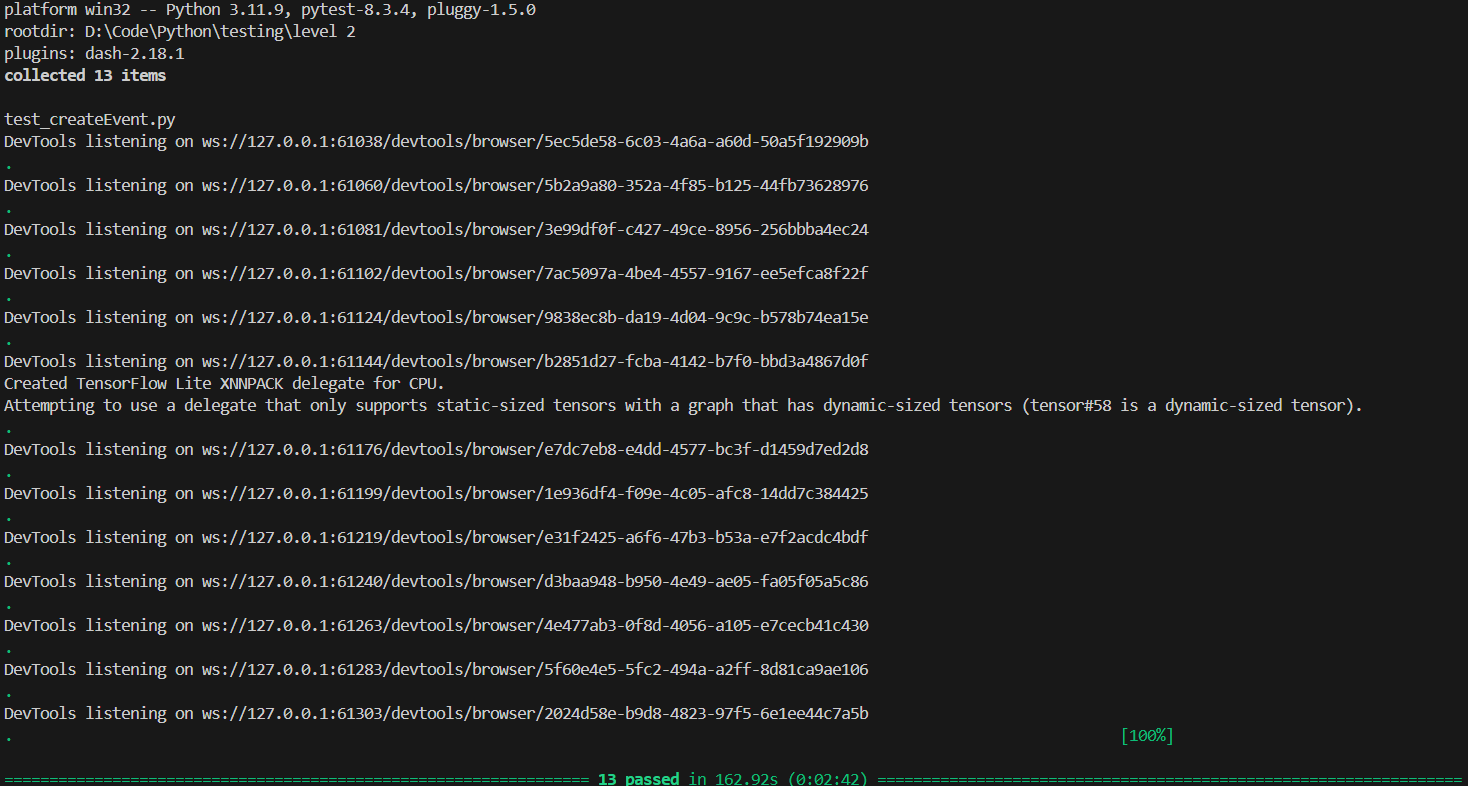
\includegraphics[width=0.8\linewidth]{image/results-create-event-lv2.png}
    \caption{Kết quả kiểm thử chức năng Create Event ở Level 2}
    \label{fig:enter-label}
\end{figure}
\subsection{Change Password}
\subsubsection{Level 1}
\begin{figure}[H]
    \centering
    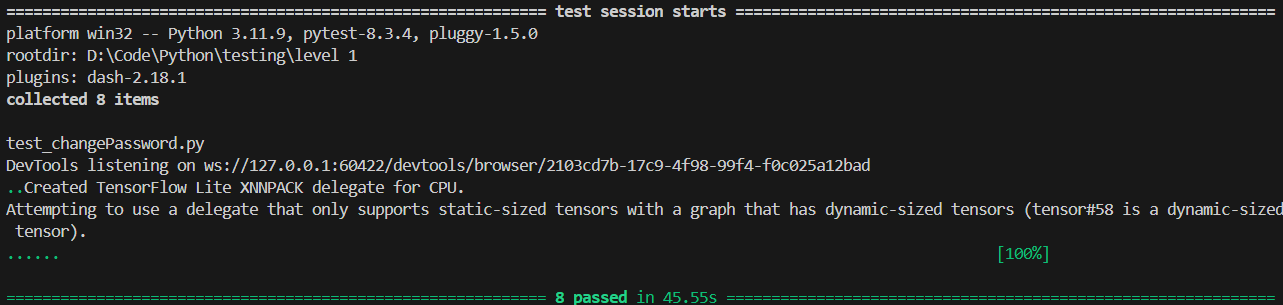
\includegraphics[width=0.8\linewidth]{image/results-change-password-lv1.png}
    \caption{Kết quả kiểm thử chức năng Change Password ở Level 1}
    \label{fig:enter-label}
\end{figure}
\subsubsection{Level 2}
\begin{figure}[H]
    \centering
    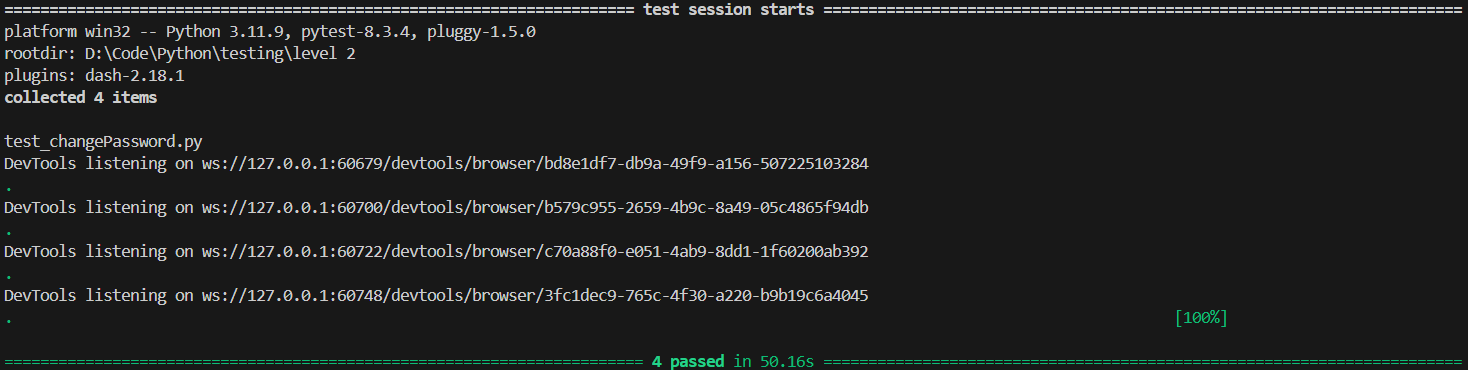
\includegraphics[width=0.8\linewidth]{image/results-change-password-lv2.png}
    \caption{Kết quả kiểm thử chức năng Change Password ở Level 2}
    \label{fig:enter-label}
\end{figure}



\subsection{Create Event}
\subsubsection{Level 1}
\begin{figure}[H]
    \centering
    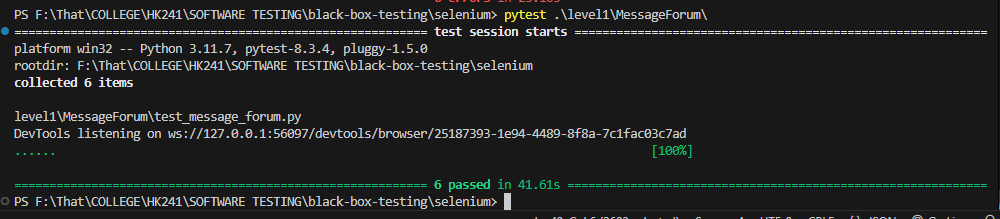
\includegraphics[width=0.8\linewidth]{image/message-forum-lv1.png}
    \caption{Kết quả kiểm thử chức năng Message Forum ở Level 1}
    \label{fig:enter-label}
\end{figure}
\subsubsection{Level 2}
\begin{figure}[H]
    \centering
    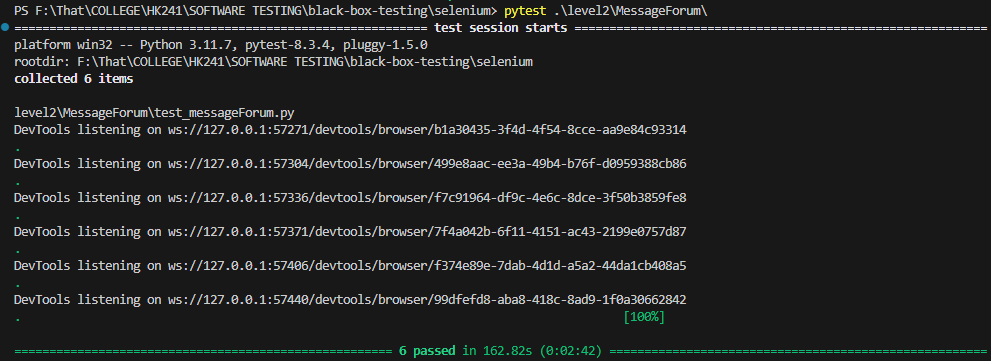
\includegraphics[width=0.8\linewidth]{image/message-forum-lv2.png}
    \caption{Kết quả kiểm thử chức năng Message Forum ở Level 2}
    \label{fig:enter-label}
\end{figure}
\subsection{Change Password}
\subsubsection{Level 1}
\begin{figure}[H]
    \centering
    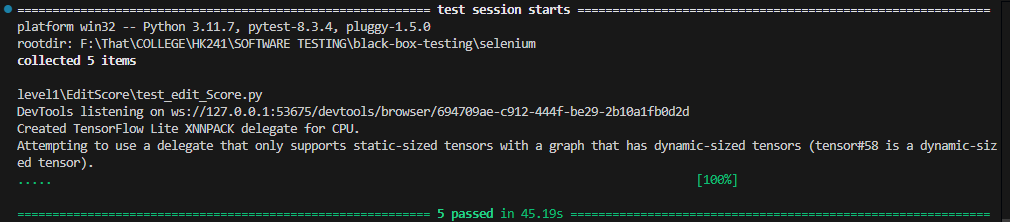
\includegraphics[width=0.8\linewidth]{image/edit-score-lv1.png}
    \caption{Kết quả kiểm thử chức năng Edit Score ở Level 1}
    \label{fig:enter-label}
\end{figure}
\subsubsection{Level 2}
\begin{figure}[H]
    \centering
    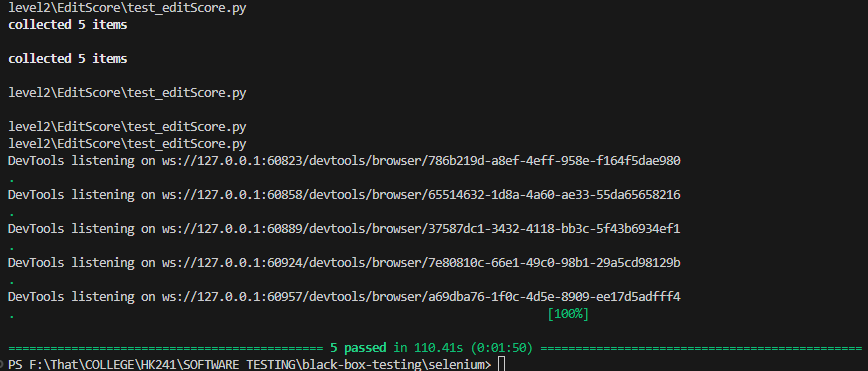
\includegraphics[width=0.8\linewidth]{image/edit-score-lv2.png}
    \caption{Kết quả kiểm thử chức năng Edit Score ở Level 2}
    \label{fig:enter-label}
\end{figure}


\end{document}
